\chapter{Model Evaluation}
\label{ch:evaluation}

\section{Classification Metrics}
\label{sec:metriques_classif}

\index{accuracy}\index{precision}\index{recall}\index{F1-score}

\begin{definition}[Confusion Matrix]
\index{confusion matrix}
The \textbf{confusion matrix} summarizes the predictions of a binary classifier into four categories:
\begin{itemize}
    \item \textbf{True positives} (TP): correctly predicted as positive.
    \item \textbf{False positives} (FP): incorrectly predicted as positive (type I error).
    \item \textbf{True negatives} (TN): correctly predicted as negative.
    \item \textbf{False negatives} (FN): incorrectly predicted as negative (type II error).
\end{itemize}
\end{definition}

\begin{center}
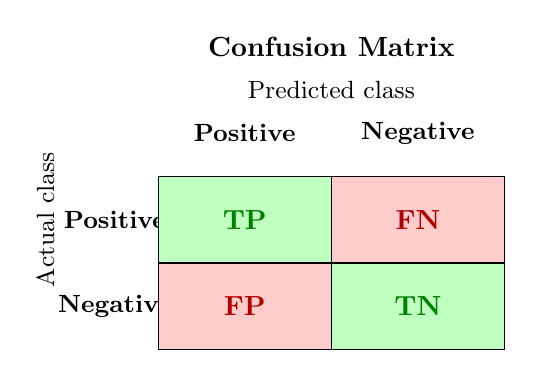
\begin{tikzpicture}[scale=1.1]
    % Title
    \node[font=\bfseries] at (2.5, 3.5) {Confusion Matrix};
    \node[font=\small, rotate=90] at (-0.8, 1.5) {Actual class};
    \node[font=\small] at (2.5, 3) {Predicted class};

    % Headers
    \node[font=\small\bfseries] at (1.5, 2.5) {Positive};
    \node[font=\small\bfseries] at (3.5, 2.5) {Negative};
    \node[font=\small\bfseries] at (0, 1.5) {Positive};
    \node[font=\small\bfseries] at (0, 0.5) {Negative};

    % Cells
    \fill[green!25] (0.5, 1) rectangle (2.5, 2);
    \draw (0.5, 1) rectangle (2.5, 2);
    \node[font=\bfseries, green!50!black] at (1.5, 1.5) {TP};

    \fill[red!20] (2.5, 1) rectangle (4.5, 2);
    \draw (2.5, 1) rectangle (4.5, 2);
    \node[font=\bfseries, red!70!black] at (3.5, 1.5) {FN};

    \fill[red!20] (0.5, 0) rectangle (2.5, 1);
    \draw (0.5, 0) rectangle (2.5, 1);
    \node[font=\bfseries, red!70!black] at (1.5, 0.5) {FP};

    \fill[green!25] (2.5, 0) rectangle (4.5, 1);
    \draw (2.5, 0) rectangle (4.5, 1);
    \node[font=\bfseries, green!50!black] at (3.5, 0.5) {TN};
\end{tikzpicture}
\end{center}

\begin{definition}[Classification Metrics]
From the confusion matrix, we define:
\begin{align}
\text{Accuracy} &= \frac{TP + TN}{TP + TN + FP + FN} \\[6pt]
\text{Precision} &= \frac{TP}{TP + FP} \quad \text{(among predicted positives)} \\[6pt]
\text{Recall} &= \frac{TP}{TP + FN} \quad \text{(among actual positives)} \\[6pt]
\text{F1-score} &= 2 \cdot \frac{\text{Precision} \times \text{Recall}}{\text{Precision} + \text{Recall}}
\end{align}
\end{definition}

\begin{intuition}
\begin{itemize}
    \item \textbf{Precision} answers: ``Among those I declared sick, how many are truly sick?''
    \item \textbf{Recall} answers: ``Among the truly sick, how many did I detect?''
    \item The \textbf{F1-score} is the harmonic mean of both, useful when classes are imbalanced.
\end{itemize}
\end{intuition}

\subsection{Example with the Titanic}

\begin{codeblock}[title=\textbf{Python}]
\begin{minted}{python}
import seaborn as sns
import pandas as pd
from sklearn.model_selection import train_test_split
from sklearn.ensemble import RandomForestClassifier
from sklearn.metrics import (classification_report,
                             confusion_matrix, accuracy_score)

# Titanic data preparation
titanic = sns.load_dataset('titanic').dropna(subset=['age', 'fare'])
titanic['sex_num'] = titanic['sex'].map({'male': 0, 'female': 1})
X = titanic[['pclass', 'age', 'fare', 'sex_num']]
y = titanic['survived']

X_train, X_test, y_train, y_test = train_test_split(
    X, y, test_size=0.3, random_state=42, stratify=y
)

# Training
rf = RandomForestClassifier(n_estimators=100, random_state=42)
rf.fit(X_train, y_train)
y_pred = rf.predict(X_test)

# Confusion matrix
print("Confusion matrix:")
print(confusion_matrix(y_test, y_pred))
print()
print("Classification report:")
print(classification_report(y_test, y_pred, target_names=['Deceased', 'Survived']))
\end{minted}
\end{codeblock}

\begin{codeoutput}
\begin{minted}{text}
Confusion matrix:
[[103  19]
 [ 25  67]]

Classification report:
              precision    recall  f1-score   support

    Deceased       0.80      0.84      0.82       122
    Survived       0.78      0.73      0.75        92

    accuracy                           0.79       214
   macro avg       0.79      0.79      0.79       214
weighted avg       0.79      0.79      0.79       214
\end{minted}
\end{codeoutput}

\begin{warning}
\textbf{Accuracy} alone is misleading on imbalanced data. If 95\% of emails are legitimate, a model that always predicts ``legitimate'' will have 95\% accuracy but will detect no spam!
\end{warning}

\section{ROC Curve and AUC}
\label{sec:roc_auc}

\index{ROC curve}\index{AUC}

\begin{definition}[ROC Curve]
The \textbf{ROC curve} (\textit{Receiver Operating Characteristic}) plots the \textbf{true positive rate} (recall) against the \textbf{false positive rate} for different decision thresholds. The \textbf{AUC} (\textit{Area Under the Curve}) measures the area under this curve: $\text{AUC} \in [0, 1]$.
\end{definition}

\begin{codeblock}[title=\textbf{Python}]
\begin{minted}{python}
from sklearn.metrics import roc_auc_score, roc_curve

# Predicted probabilities
y_proba = rf.predict_proba(X_test)[:, 1]

# AUC
auc = roc_auc_score(y_test, y_proba)
print(f"AUC: {auc:.4f}")

# ROC curve points
fpr, tpr, thresholds = roc_curve(y_test, y_proba)
print(f"Number of thresholds: {len(thresholds)}")
print(f"FPR (first 5): {fpr[:5].round(3)}")
print(f"TPR (first 5): {tpr[:5].round(3)}")
\end{minted}
\end{codeblock}

\begin{codeoutput}
\begin{minted}{text}
AUC: 0.8575
Number of thresholds: 18
FPR (first 5): [0.    0.    0.008 0.016 0.041]
TPR (first 5): [0.    0.011 0.065 0.13  0.239]
\end{minted}
\end{codeoutput}

\begin{remark}
A random classifier has an AUC of $0.5$ (diagonal). A perfect classifier has an AUC of $1.0$. In general, an AUC $> 0.8$ is considered good.
\end{remark}

\section{Regression Metrics}
\label{sec:metriques_regression}

\index{MAE}\index{MSE}\index{RMSE}

\begin{definition}[Regression Metrics]
Let $\hat{y}_i$ be the predictions and $y_i$ the actual values:
\begin{align}
\text{MAE} &= \frac{1}{n}\sum_{i=1}^{n}|y_i - \hat{y}_i| \\[6pt]
\text{MSE} &= \frac{1}{n}\sum_{i=1}^{n}(y_i - \hat{y}_i)^2 \\[6pt]
\text{RMSE} &= \sqrt{\text{MSE}} \\[6pt]
R^2 &= 1 - \frac{\sum(y_i - \hat{y}_i)^2}{\sum(y_i - \bar{y})^2}
\end{align}
\end{definition}

\begin{codeblock}[title=\textbf{Python}]
\begin{minted}{python}
from sklearn.metrics import mean_absolute_error, mean_squared_error, r2_score
from sklearn.linear_model import LinearRegression
import numpy as np

tips = sns.load_dataset('tips')
X_reg = tips[['total_bill', 'size']]
y_reg = tips['tip']

X_train, X_test, y_train, y_test = train_test_split(
    X_reg, y_reg, test_size=0.3, random_state=42
)

reg = LinearRegression()
reg.fit(X_train, y_train)
y_pred = reg.predict(X_test)

print(f"MAE:  {mean_absolute_error(y_test, y_pred):.4f}")
print(f"MSE:  {mean_squared_error(y_test, y_pred):.4f}")
print(f"RMSE: {np.sqrt(mean_squared_error(y_test, y_pred)):.4f}")
print(f"R\u00b2:   {r2_score(y_test, y_pred):.4f}")
\end{minted}
\end{codeblock}

\begin{codeoutput}
\begin{minted}{text}
MAE:  0.7359
MSE:  1.0940
RMSE: 1.0459
R²:   0.4616
\end{minted}
\end{codeoutput}

\section{Advanced Cross-Validation}
\label{sec:cv_avancee}

\index{stratified cross-validation}\index{StratifiedKFold}

\begin{definition}[Stratified Cross-Validation]
\textbf{Stratified cross-validation}\index{stratified cross-validation} preserves the \textbf{class proportions} in each fold. It is recommended for classification, especially with imbalanced classes.
\end{definition}

\begin{codeblock}[title=\textbf{Python}]
\begin{minted}{python}
from sklearn.model_selection import cross_val_score, StratifiedKFold

# 5-fold stratified cross-validation
skf = StratifiedKFold(n_splits=5, shuffle=True, random_state=42)

rf = RandomForestClassifier(n_estimators=100, random_state=42)
scores = cross_val_score(rf, X, y, cv=skf, scoring='f1')

print(f"F1-scores per fold: {scores.round(4)}")
print(f"Mean F1: {scores.mean():.4f} (+/- {scores.std():.4f})")
\end{minted}
\end{codeblock}

\begin{codeoutput}
\begin{minted}{text}
F1-scores per fold: [0.7273 0.7143 0.7500 0.7647 0.7692]
Mean F1: 0.7451 (+/- 0.0207)
\end{minted}
\end{codeoutput}

\section{Hyperparameter Optimization}
\label{sec:gridsearch}

\index{GridSearchCV}\index{hyperparameters}

\begin{definition}[GridSearchCV]
\py{GridSearchCV} performs an \textbf{exhaustive search} over a grid of hyperparameters, evaluating each combination using cross-validation.
\end{definition}

\begin{codeblock}[title=\textbf{Python}]
\begin{minted}{python}
from sklearn.model_selection import GridSearchCV
from sklearn.ensemble import RandomForestClassifier

# Define the grid
param_grid = {
    'n_estimators': [50, 100, 200],
    'max_depth': [3, 5, 10, None],
    'min_samples_split': [2, 5]
}

grid_search = GridSearchCV(
    RandomForestClassifier(random_state=42),
    param_grid,
    cv=5,
    scoring='accuracy',
    n_jobs=-1
)
grid_search.fit(X_train, y_train)

print(f"Best parameters: {grid_search.best_params_}")
print(f"Best score (CV): {grid_search.best_score_:.4f}")
print(f"Test score:      {grid_search.score(X_test, y_test):.4f}")
\end{minted}
\end{codeblock}

\begin{codeoutput}
\begin{minted}{text}
Best parameters: {'max_depth': 5, 'min_samples_split': 5, 'n_estimators': 100}
Best score (CV): 0.8006
Test score:      0.7944
\end{minted}
\end{codeoutput}

\begin{bestpractice}
Use \py{GridSearchCV} to find the best hyperparameters systematically. For large grids, prefer \py{RandomizedSearchCV}\index{RandomizedSearchCV} which randomly samples a subset of combinations.
\end{bestpractice}

\section{Learning Curves}
\label{sec:learning_curves}

\index{learning curve}

\begin{definition}[Learning Curve]
A \textbf{learning curve} plots the training and validation scores as a function of the \textbf{training set size}. It helps diagnose overfitting or underfitting.
\end{definition}

\begin{codeblock}[title=\textbf{Python}]
\begin{minted}{python}
from sklearn.model_selection import learning_curve
import numpy as np

train_sizes, train_scores, val_scores = learning_curve(
    RandomForestClassifier(n_estimators=50, random_state=42),
    X, y, cv=5,
    train_sizes=np.linspace(0.1, 1.0, 5),
    scoring='accuracy'
)

print("Size   | Train score | Valid. score")
print("-" * 42)
for size, tr, va in zip(train_sizes, train_scores.mean(axis=1),
                         val_scores.mean(axis=1)):
    print(f"  {size:4d} |    {tr:.4f}   |    {va:.4f}")
\end{minted}
\end{codeblock}

\begin{codeoutput}
\begin{minted}{text}
Size   | Train score | Valid. score
------------------------------------------
    52 |    0.9962   |    0.6930
   104 |    0.9923   |    0.7451
   157 |    0.9936   |    0.7686
   210 |    0.9924   |    0.7851
   263 |    0.9924   |    0.7944
\end{minted}
\end{codeoutput}

\begin{intuition}
\begin{itemize}
    \item If training and validation scores are \textbf{close and low}: underfitting (increase complexity).
    \item If the training score is \textbf{high} but the validation score is \textbf{low}: overfitting (reduce complexity or increase data).
    \item If both scores \textbf{converge to a high value}: good model.
\end{itemize}
\end{intuition}

\section{Exercises}

\begin{exercise}[$\star$]
Manually compute the precision, recall, and F1-score from the following confusion matrix:
\[
\begin{pmatrix} 45 & 5 \\ 10 & 40 \end{pmatrix}
\]
Verify your results with scikit-learn.
\end{exercise}

\begin{exercise}[$\star$]
Explain in which cases recall is preferred over precision. Give two concrete examples.
\end{exercise}

\begin{exercise}[$\star\star$]
On the Iris dataset, train a KNN and plot the ROC curve (one-vs-rest) for each class. Compute the AUC for each class.
\end{exercise}

\begin{exercise}[$\star\star$]
Use \py{GridSearchCV} to optimize the hyperparameters of a \py{KNeighborsClassifier} on the \texttt{penguins} dataset from seaborn. Test $k \in \{1, 3, 5, 7, 9, 11\}$ and distance metrics \py{('euclidean', 'manhattan')}.
\end{exercise}

\begin{exercise}[$\star\star\star$]
On the Titanic dataset, compare three models (logistic regression, random forest, KNN) using 10-fold stratified cross-validation. For each model, report the mean accuracy, precision, recall, and F1-score. Which model do you recommend and why?
\end{exercise}

\begin{exercise}[$\star\star\star$]
Plot the learning curves for a decision tree with \py{max_depth=2}, \py{max_depth=5}, and \py{max_depth=None} on the Titanic dataset. Interpret the results in terms of the bias-variance tradeoff.
\end{exercise}

\begin{keyformulas}
\textbf{Summary of Chapter~\ref{ch:evaluation}}
\begin{itemize}
    \item \textbf{Confusion matrix}: TP, FP, TN, FN.
    \item \textbf{Accuracy}: $(TP + TN) / N$, misleading if classes are imbalanced.
    \item \textbf{Precision}: $TP / (TP + FP)$, \textbf{Recall}: $TP / (TP + FN)$.
    \item \textbf{F1-score}: $2 \cdot \frac{\text{Precision} \times \text{Recall}}{\text{Precision} + \text{Recall}}$.
    \item \textbf{ROC curve / AUC}: TPR vs.\ FPR, $\text{AUC} \in [0, 1]$.
    \item \textbf{Regression}: MAE, MSE, RMSE, $R^2$.
    \item \textbf{GridSearchCV}: exhaustive hyperparameter search with CV.
    \item \textbf{Learning curve}: overfitting/underfitting diagnosis.
\end{itemize}
\end{keyformulas}
